\chapter{Popcorn Linux Background}
Our replication prototype is built on top of Popcorn Linux ~\cite{barbalace2014popcorn}. It is a multi-kernel OS which allows a multi-core system to boot multiple Linux kernels. In this project, we leverage this architecture to achieve inter-machine replication. The replicated applications will run on different kernel instances and Popcorn Linux provides strong isolation of the resources on the machine.
% talk about multi-kernel boot here
% Put a plot of popcorn architecture here
\section{Hardware Partitioning}
In Popcorn Linux, hardware resources are partitioned into arbitrary divisions, as shown in Figure~\ref{f:popcorn_arch}, each booted kernel instance can have the full control of its own partition. In general, the CPU cores and memory can be splitted into different partitions, each kernel can have its own dedicated CPU cores and memory. The hardware partitioning provides a very strong isolation for all the kernels and the applications running on them, which is ideal for our intra-machine fault tolerance model. Especially when the partition is done based on NUMA zones, a critical hardware error happens on one kernel's hardware partition can hardly get propagated to another.

\begin{figure}[!ht]
\centering
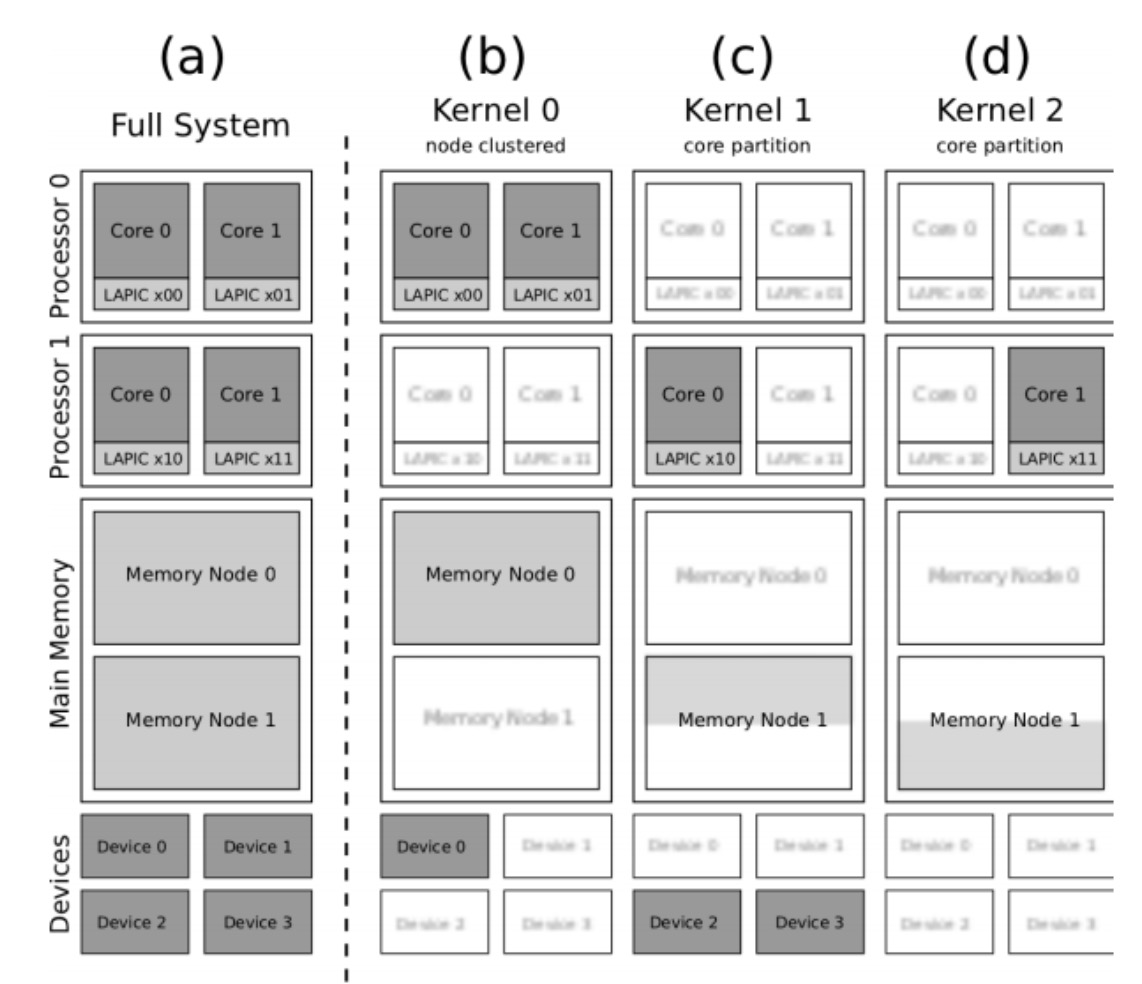
\includegraphics[width=.6\columnwidth]{figures/popcorn_arch}
 \caption{Popcorn Linux hardware partitioning}
 \label{f:popcorn_arch}
\end{figure}

\section{Inter-Kernel Messaging Layer}
Popcorn Linux comes with a high efficient messaging layer for inter-kernel communication ~\cite{shelton2013popcorn}. From the implementation perspective, the messaging passing is basically just a set of memory copy operations between the address space of the sender kernel and receiver kernel. As a result, the cost of sending a message is very low (under 5us). The replication protocol developed in this project heavily leverage Popcorn’s messaging layer.
% Important fact: messaging layer is strictly FIFO

\section{Popcorn Namespace}
In Linux, namespaces are used for creating isolated execution environment for applications. Popcorn Linux implemented a new Linux namespace in order to isolate normal applications and replicated applications. Applications inside Popcorn Namespace will utilize our replication service, once the user enters the Popcorn namespace, all the applications that run inside it will be replicated to the secondary kernel.

\subsection{Replicated Execution}
When a user launches an application inside the namespace, Popcorn Linux will gather all the information for launching this application (full executable path, environment variables, etc) and send it to the secondary replica. On the secondary, a kernel thread will be spawned with all the information it received, to create an identical process as the one in the primary replica. This makes launching the replicated application to be transparent to the user.

\subsection{FT PID}
In order to match the replicated tasks, Popcorn Linux introduced an extra field to Linux's task\_struct called ft\_pid. As shown in Figure~\ref{f:ft_pid}, ft\_pid is an array of IDs in order to match the tasks on both sides, other parts in the system use ft\_pid to synchronize the execution of tasks on both sides with the same ft\_pid. Popcorn Linux makes sure that the creation of a process/thread is deterministic on both sides, so that all child processes/threads can be matched properly on both sides.
\begin{figure}[!ht]
\centering
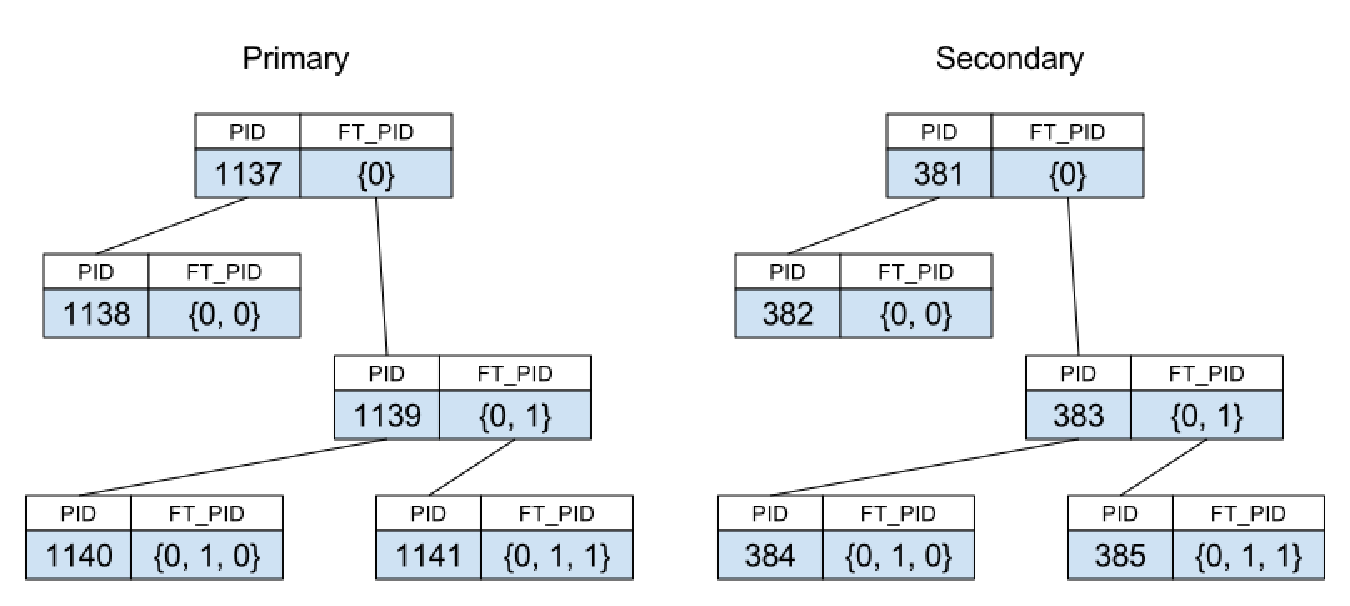
\includegraphics[width=.9575\columnwidth]{figures/ft_pid}
 \caption{An example of ft\_pid}
 \label{f:ft_pid}
\end{figure}

\section{Network Stack Replication}
% Important fact: accept sequence is same on primary and replica
The TCP stack in Linux is intrinsically non-deterministic. Given the same network stream, the internal state of TCP stack might end up with different states. For example, for read/write operations, the TCP stack may return a non-predictable number of bytes to the application reading from the socket, which might in turn leads to different states in the replicas.

Based on the idea of FT-TCP~\cite{zagorodnov2009practical}, Popcorn Linux comes with the network stack replication to eliminate this kind of non-determinism during the replication of network applications. On the inbound path of Linux's network stack, all the TCP traffic that are related to an active Popcorn namespace will be copied to the secondary. All read/write/accept/listen/close system calls that are related to a replicated socket will be synchronized between two kernel instances. Any event that will cause the TCP state to change will be synchronized inside the stack(SYN, FIN, etc). While for the events that doesn't affect the TCP state (normal read and write), the secondary simply bypasses its own TCP stack and simply copies the system call output of the primary.

In general, the network stack replication service provides following important functionalities for replicating network applications:
\begin{itemize}
\item The internal state of every replicated socket is synchronized.
\item Read and write operations can have consistent output across all replicas, in terms of size and content.
\item Upon accept is returned, it is made sure that both replicas are returning the same socket with the same TCP stream.
\end{itemize}